\documentclass{article}
\usepackage{enumitem}
\usepackage[cachedir=minted_cache]{minted}
\usepackage{graphicx}
\graphicspath{ {./img/} }
\usepackage[margin=1in]{geometry} %used to set the margins
\setcounter{secnumdepth}{0} %used to get rid of section numbers
\title{Lab 7: Pattern Matching}
\author{Michael Morikawa}
\date{\today}


\begin{document}
\maketitle
\section{Lab Questions}
\begin{enumerate}[label=\textbf{Question \arabic*}]
    \item Are there any situations where BM better than KMP? Explain.\\
          \textbf{
              Yes, if the pattern is short and doesn't have any prefix/suffix in common within its substrings.
          }
    \item  Is Brute Force Pattern Matching with BM’s looking-glass heuristic
          always better than original Brute Force Pattern Matching? Explain.\\
          \textbf{
              It will not always be better than the original brute force algorithm. This is because it is possible for a mismatch to only occur at the
              beginning of a pattern and thus the looking glass heuristic will take more comparisons.
          }


\end{enumerate}

\section{Source Code}

\subsection{main.cpp}
\inputminted{c++}{../src/main.cpp}

\section{Output}
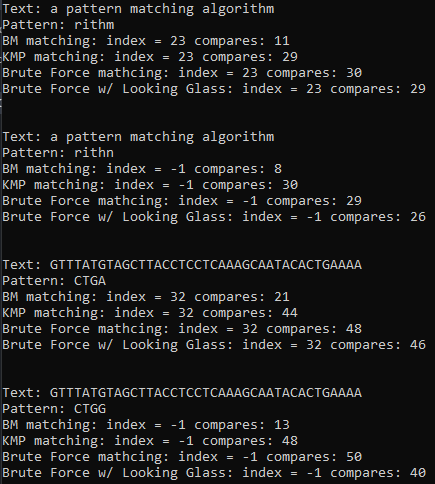
\includegraphics[]{output.png}

\end{document}